\section{方法描述} % 陈克勤

\subsection{基础方法}

基础方法将该任务建模为文本分类问题。使用BERT模型进行微调来解决。

\subsubsection{BERT模型}

BERT是基于Transformer架构的预训练模型\cite{devlin2019bert}。通过在大型语料库上的进行遮罩语言建模和下一句预测两个任务的无监督预训练,BERT拥有了强大的泛化能力。从而只需要在下游任务上进行少量的微调迭代即可取得不错的性能。

BERT由许多层的Transformer编码器\cite{vaswani2017attention}堆叠而成,每个编码器由多头自注意力和前馈网络组成。记$x^l=\{x_1^l,\dots,x_N^l\}$为第$l$层的特征,则第$l+1$层的特征$x^{l+1}$为:
\begin{equation}
    x^{l+1} = \text{FNN}(\text{MultiHead}(x^l))
\end{equation}

自注意力可以用来建模序列中元素对该序列中其他元素的依赖关系,结构如图~\ref{fig:selfatten}~(左)所示。BERT中使用的自注意力首先通过线性层将原始输入映射到三个不同的空间。即$[Q,K,V]=[W_q,W_k,W_v]\cdot X$。再使用乘法注意力来计算输出。多头自注意力并行使用多个自注意力,并将其各自的结果进行拼接,作为最终输出。结构如图~\ref{fig:selfatten}~(右)所示。整体公式如下:
\begin{equation}
    \begin{aligned}
    \text{MultiHead}(X) &= [\text{head}_1,\dots,\text{head}_n]W^O \\
    \text{head}_i &= \text{Self-Attention}(X) \quad \forall 1\leq i\leq n \\
    \text{Self-Attention}(X) &= \text{Attention}(W_qX,W_kX,W_vX) \\
    \text{Attention}(Q,K,V) &= \text{Softmax}(\frac{QK^T}{\sqrt{d}})V 
\end{aligned}
\end{equation}

\begin{figure}
    \centering
    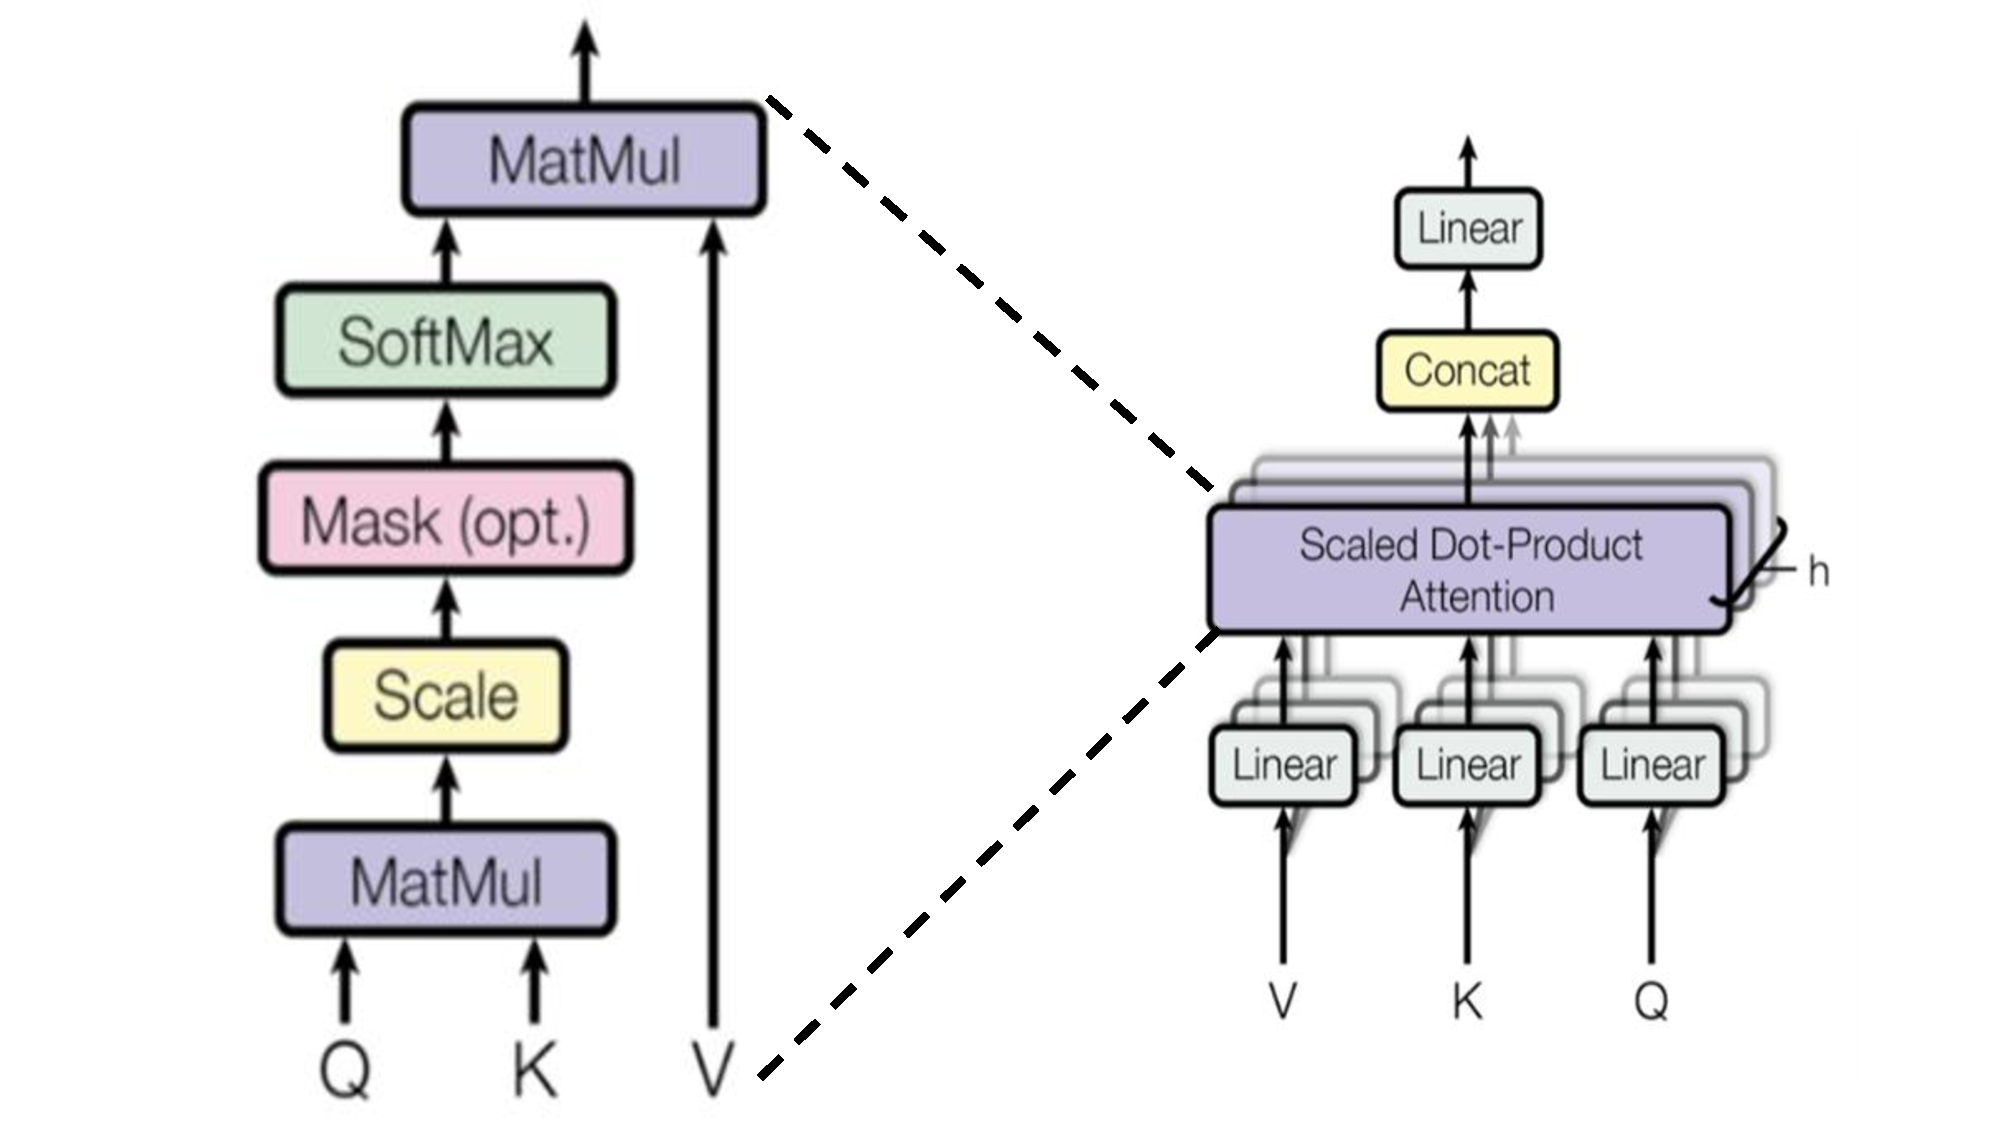
\includegraphics[width=.8\textwidth]{figs/atten.pdf}
    \caption{多头自注意力结构图\cite{vaswani2017attention}}
    \label{fig:selfatten}
\end{figure}

前馈网络即由简单的线性层和残差层构成。公式如下,其中act\_fn为激活函数,通常取gelu函数。
\begin{equation}
    \text{FNN}(X) = X + W_{f_2}\text{act\_fn}(W_{f_1}X)
\end{equation}

对于文本分类任务,通常在句子前添加特殊单词[CLS]作为句子整体的表示,微调时取BERT模型最后一层的[CLS]表示进行下游任务的训练。

\subsubsection{损失函数}

假设训练集中包含着$T$个训练样本$(x_t,y_t)$。对于分类问题,通常我们使用交叉熵损失函数优化模型参数,同时也使用权重衰减来正则化模型:
\begin{equation}
     \mathcal{L}(\hat{y},y)=-\sum_{i=1}^T\sum_{j=1}^Cy_i^j\log(\hat{y}_i^j)+\lambda\sum_{\theta\in\Theta}\Vert\theta\Vert_2^2
\end{equation}
其中$y_i^j$代表真实类别,$\hat{y}_i^j$代表预测类别,$C=2$,$\Theta$对应全部的可训练参数,$\lambda$控制权重衰减正则项对训练过程的影响程度。

\subsection{去偏方法}

我们尝试基于不变解释\cite{chang2020invariant}来构建去偏的恶意言论检测模型。解释是指从输入特征中选取的一个子集,仅通过该特征子集便足够检测出目标。在恶意言论检测任务中,解释可以包含对目标检测有帮助的一切特征,如带有攻击性的句子或词汇,或者指代少数群体的词汇(这部分对检测有帮助往往是因为训练数据有偏)。不变解释是指在不同环境下,该特征子集都可以稳定检测出目标。通过学习不变解释,便可以从有偏数据中过滤出无偏特征,从而得到去偏的恶意言论检测模型。

\subsubsection{问题形式化}

给定输入输出对$(\textbf{\textit{X}},Y)$,一段语句$\textbf{\textit{X}}$,可以被分为$X_1,X_2,X_3$三部分。如图~\ref{fig:form}~所示。其中$X_1$为影响检测结果$Y$的特征,$X_2$为被$Y$直接影响的特征,$X_3$为其他特征。$X_1,X_2,X_3$都有可能和$Y$高度相关,但只有$X_1$才是合理的解释。为分离出$X_1$,不变解释引入了环境变量$E$,环境变量$E$影响着$X$的先验分布,从而导致从$X_2,X_3$预测$Y$的能力在不同环境下发生变化,同时从$X_1$预测的能力保持不变。即$Y$和$E$关于$X_2,x_3$条件不独立,关于$X_1$条件独立。为过滤出合理的解释$X_1$,目标函数可形式化为:
\begin{equation}
    \begin{aligned}
    \max_{m \in S} \quad & I(Y;\textbf{\textit{Z}}) \\
    \text{s.t.}\quad & \textbf{\textit{Z}} = m \odot \textbf{\textit{X}} \\
                & Y \perp E \mid \textbf{\textit{Z}}
    \end{aligned}
    \label{con:optim}
\end{equation}
其中$I(Y;\textbf{\textit{Z}})$表示$Y$和$\textbf{\textit{Z}}$的互信息。 $S$为遮罩空间,包含预设的所有可能的遮罩方案,$m$是指输入特征$\textbf{\textit{X}}$上的一个遮罩,$\odot$表示按位乘运算。根据D分离定理,当且仅当$\textbf{\textit{Z}}=[X_1,\;0,\;0]$时,有$Y \perp E \mid \textbf{\textit{Z}}$。
\begin{figure}
    \centering
    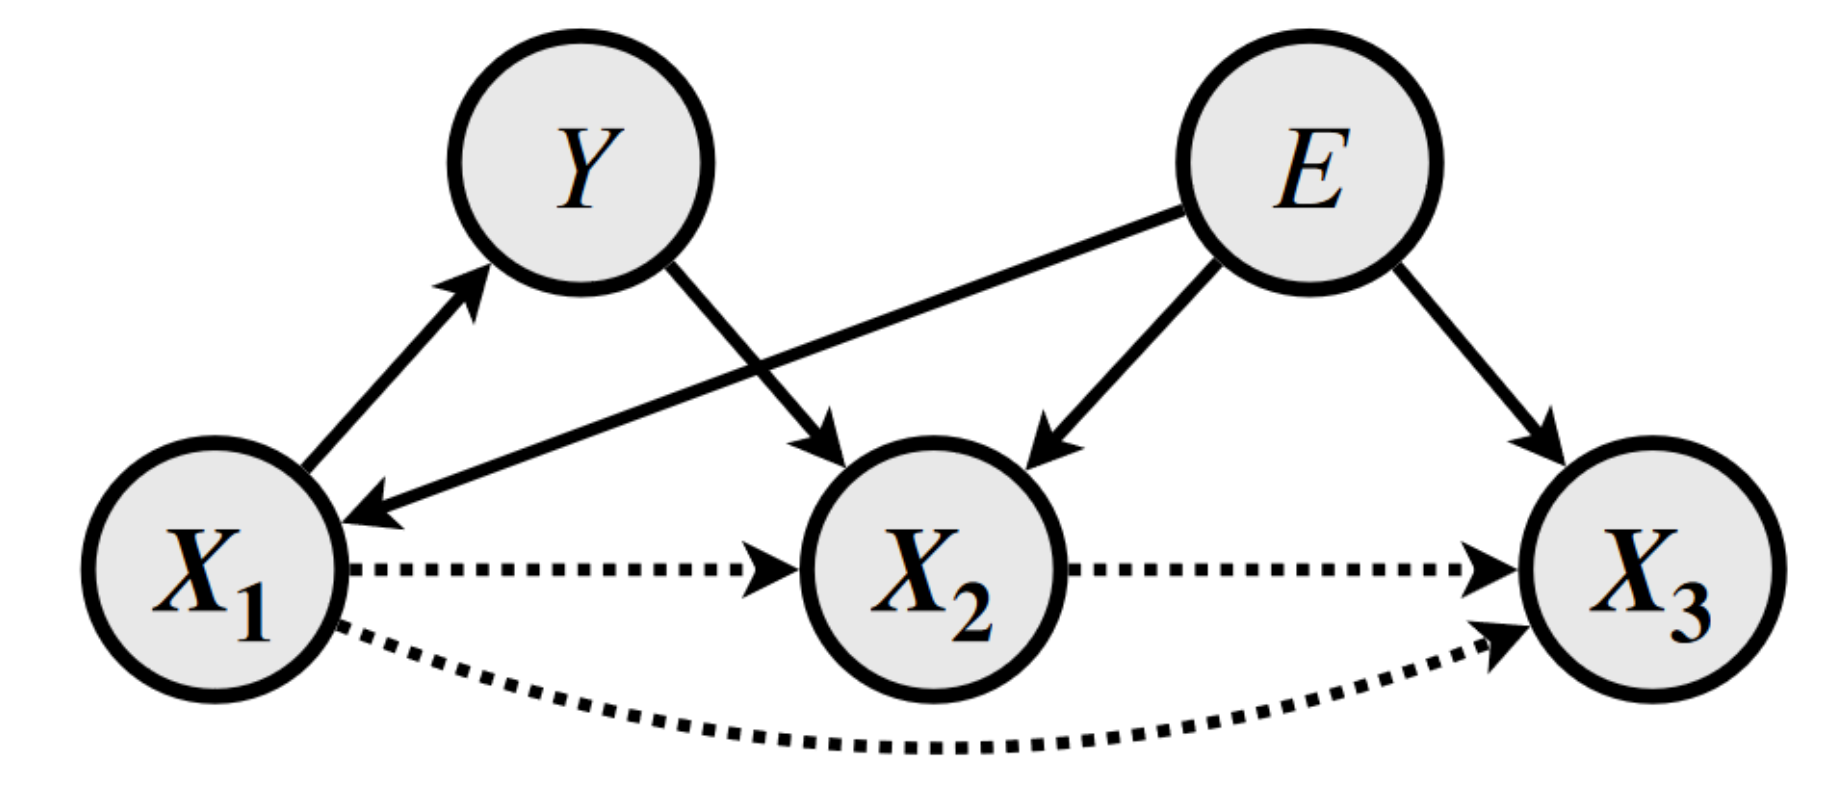
\includegraphics[width=.5\textwidth]{figs/form.png}
    \caption{不变解释示意图\cite{chang2020invariant}}
    \label{fig:form}
\end{figure}

\subsubsection{模型框架}

为解决式最优化问题(\ref{con:optim}),不变解释(InvRat)方法\cite{chang2020invariant}引入训练框架,如图~\ref{fig:invrat}~所示。该框架由三部分构成,分别是1)生成解释$\textbf{\textit{Z}}$的生成器$g(\textbf{\textit{X}})$;2)环境无关的检测器$f_i(\textbf{\textit{Z}})$;3)环境相关的检测器$f_e(\textbf{\textit{Z}},E)$。其中检测器$f_i(\textbf{\textit{Z}})$,$f_e(\textbf{\textit{Z}},E)$都用来预测$Y$,唯一的不同是是否可以访问环境$E$。记$\mathcal{L}(Y;f)$为单个样例上的交叉熵损失函数。则检测器的训练目标分布为:

\begin{equation}
    \begin{aligned}
    \mathcal{L}_i^* &= \min_{f_i(\cdot)} \mathbb{E}[\mathcal{L}(Y;f_i(\textbf{\textit{Z}}))] \\
    \mathcal{L}_e^* &= \min_{f_e(\cdot,\cdot)} \mathbb{E}[\mathcal{L}(Y;f_e(\textbf{\textit{Z}};E))]
    \end{aligned}
\end{equation}

生成器通过对输入特征$X$进行遮罩生成解释$Z$。生成器同样参与最小化环境无关预测器的训练$\mathcal{L}_i^*$。另外,还有一项用于近似约束$Y \perp E \mid \textbf{\textit{Z}}$的正则项$\lambda_{\text{diff}} \; h(\mathcal{L}_i^*-\mathcal{L}_e^*)$,其中$\lambda_{\text{diff}} > 0$为正则项系数,$h(t)$为单调增的凸函数。关于该正则项的理论分析,请参阅原论文\cite{chang2020invariant}。

\begin{figure}
    \centering
    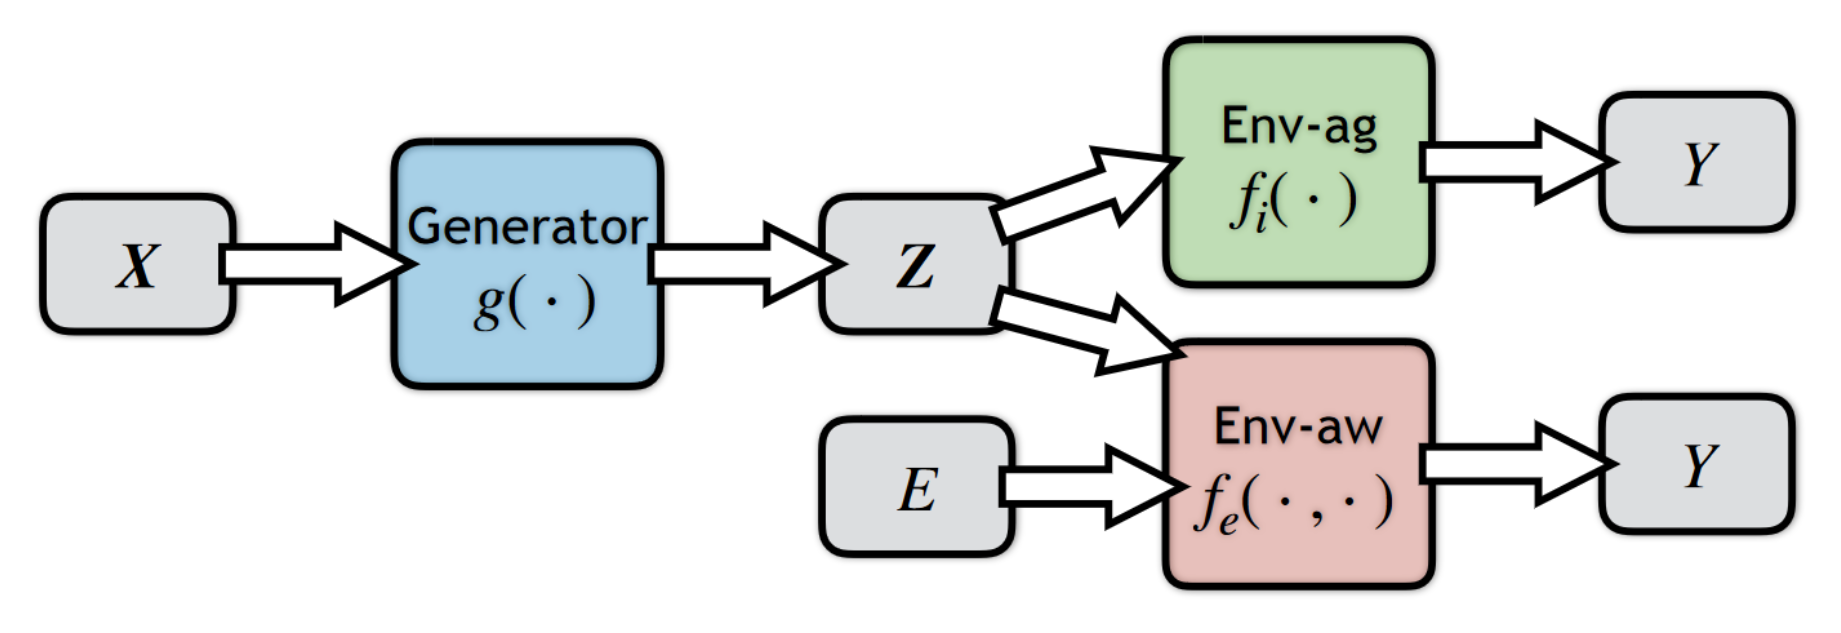
\includegraphics[width=.7\textwidth]{figs/invrat_model.png}
    \caption{不变解释框架图\cite{chang2020invariant}}
    \label{fig:invrat}
\end{figure}

\subsubsection{解释提取}

最优化问题(\ref{con:optim})中的遮罩空间$S$,需要满足稀疏性约束和连续性约束。稀疏性约束要求生成的解释$\textbf{\textit{Z}}$只包含少部分特征;连续性约束要求所截取的特征片段要尽可能连续。这符合人类理解自然语言的特点:一段话是否有恶意,仅仅通过少部分单词,语句就能反应出;相比于任意选取的单词,词组和语句片段能保留更多结构信息,更容易理解。据此,使用两个正则项\cite{changGameTheoreticApproach2019}:

\begin{equation}
    \lambda_{\text{sparsity}}\; \mathbb{E} \left[ \left| \frac{1}{N} \Vert m \Vert_1 -\alpha \right| \right]
    + 
    \lambda_{\text{continuity}}\; \mathbb{E} \left[ \sum_{n=2}^{N} \left| m_n-m_{n-1} \right|
    \right]
\end{equation}
其中,$\lambda_{\text{sparsity}},\lambda_{\text{continuity}}>0$为正则项系数,$\alpha$为所生成遮罩$m$的目标稀疏比例。

\subsubsection{损失函数}

以上多个目标函数整体上还可以表述成最小化最大值问题的形式:

\begin{equation}
\begin{aligned}
    \min_{g(\cdot),f_i(\cdot)} \max_{f_e(\cdot)}\quad
    \mathcal{L}_i(g,f_i) &+\lambda_{\text{diff}}\;h(\mathcal{L}_i(g,f_i)-\mathcal{L}_e(g,f_e))
    \\&+\lambda_{\text{sparsity}}\; \mathbb{E} \left[ \left| \frac{1}{N} \Vert m \Vert_1 -\alpha \right| \right]
    \\&+ 
    \lambda_{\text{continuity}}\; \mathbb{E} \left[ \sum_{n=2}^{N} \left| m_n-m_{n-1} \right|
    \right]
\end{aligned}    
\end{equation}

其中
\begin{equation}
\begin{aligned}
    \mathcal{L}_{i}\left(g, f_{i}\right)&=\mathbb{E}\left[\mathcal{L}\left(Y ; f_{i}(\textbf{\textit{Z}})\right)\right]
    \\\mathcal{L}_{e}\left(g, f_{e}\right)&=\mathbb{E}\left[\mathcal{L}\left(Y ; f_{e}(\textbf{\textit{Z}}, E)\right)\right]
    \\\textbf{\textit{Z}} &= m \odot \textbf{\textit{X}}
    \\m &= g(\textbf{\textit{X}})
\end{aligned}
\end{equation}
